\section{Solution}
\subsection{Solution's fundamentals}
\begin{frame}{Proposed solution}{Solution's fundamentals}
\small
\begin{block}{\small \textbf{The underlying fundamentals of proposed solution}}
\begin{itemize}
  \item Stay points \cite{Li2008}.
  \item Event-driven systems \cite{Faison2011}.
  \item Cognitive Dynamic Systems \cite{Haykin2014,Haykin2012a,Feng2017}.
\end{itemize}
\end{block}
\end{frame}



\subsection{Solution's overview}
{\aauwavesbg%
\begin{frame}[plain]
  \begin{textblock*}{8.5cm}(4.3cm,8.3cm)
  \small
  \textbf{Architecture of proposed system solution. The global perception-action cycle, the different memory types, and the internal feedback loops are observed.}
  \end{textblock*}

  \begin{textblock*}{1cm}(12cm,9.3cm)
  \scriptsize
  \insertframenumber~/~\inserttotalframenumber
  \end{textblock*}

  \centering
  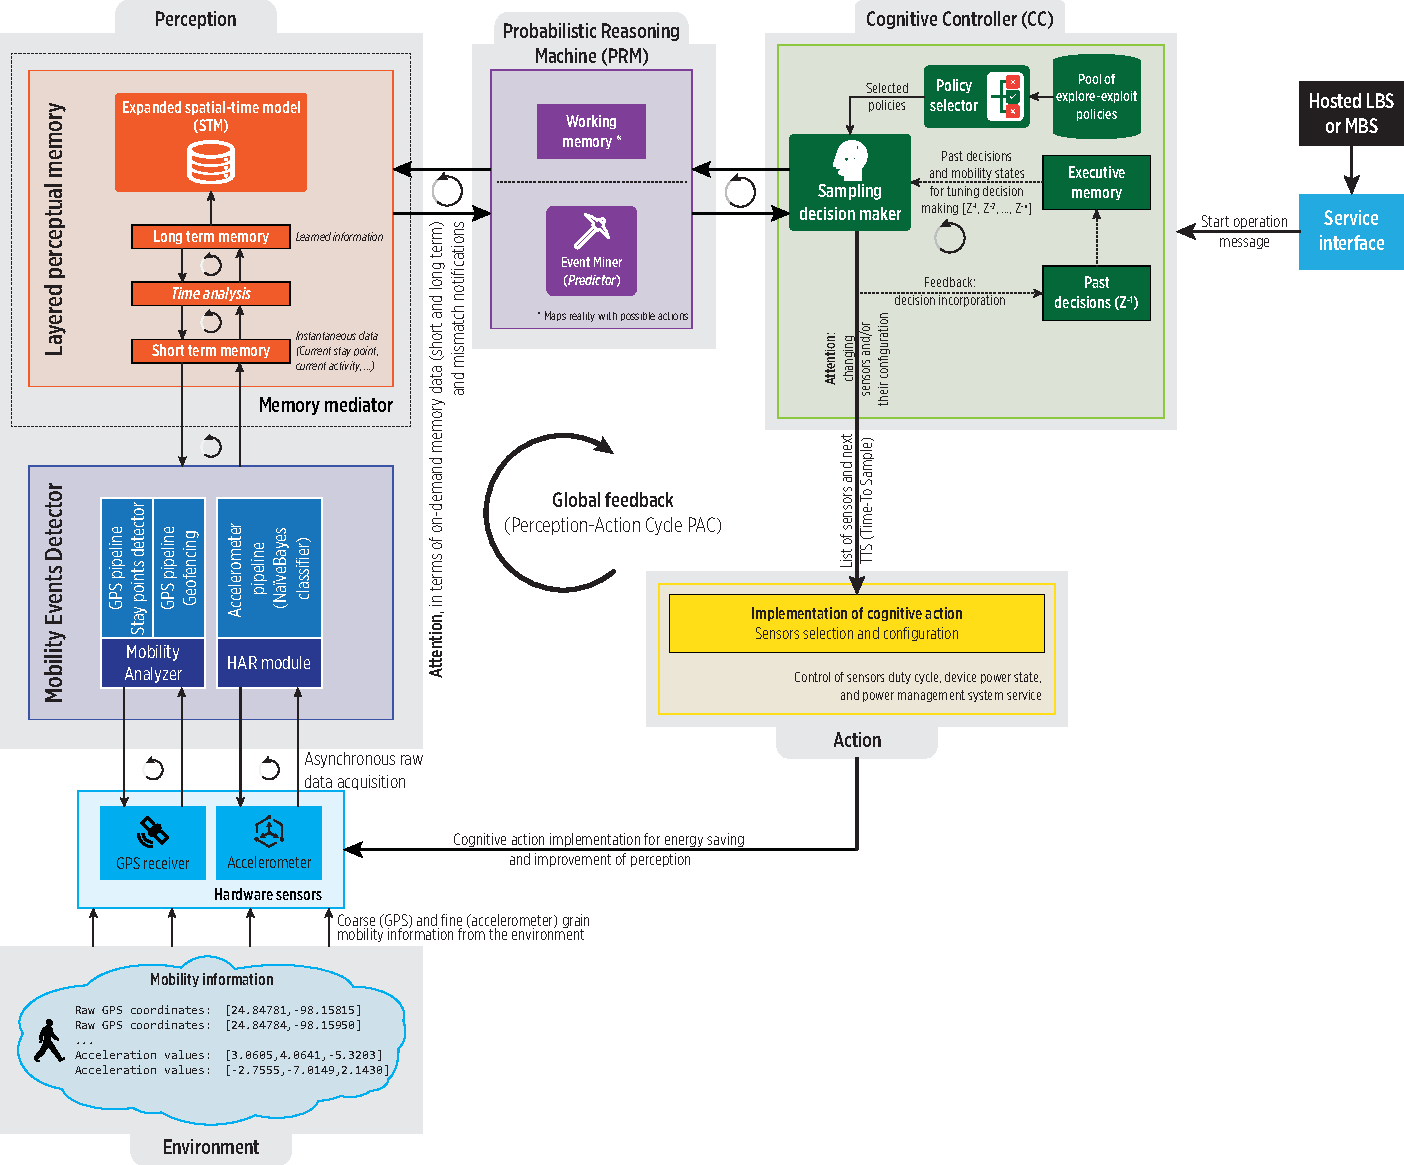
\includegraphics[width=0.98\textwidth]{vectors/inspired-cds-solution-for-slides}
  %\captionof{figure}{Architecture of proposed system solution. The global perception-action cycle and the internal loops are observed.}
\end{frame}}

\section{Schedule}
\subsection{Schedule}
\begin{frame}{Updated schedule}
\small

\begin{table}
%\cellcolor[gray]{0.3}
\definecolor{colorA}{gray}{0.85}
\definecolor{colorB}{gray}{0.95}
\definecolor{colorStep}{gray}{1}
\definecolor{colorCell}{gray}{0.3}
% \definecolor{colorCell}{HTML}{00D2CB}
\renewcommand{\arraystretch}{1.2}
\centering
\resizebox{\textwidth}{!}{%

%\fontfamily{phv}\fontsize{7.3}{9}\selectfont
\begin{tabular}{lllllllllllllll}
   &                                                                                                                             & \multicolumn{5}{c}{2017}                                                                                                                  & \multicolumn{8}{c}{2018}                                                                                                                                                                                                      \\
   \toprule
\# & \multicolumn{1}{c}{Activity}                                                                                                & \multicolumn{1}{c}{\scriptsize{Aug}}   & \multicolumn{1}{c}{\scriptsize{Sep}}   & \multicolumn{1}{c}{\scriptsize{Oct}}   & \multicolumn{1}{c}{\scriptsize{Nov}}   & \multicolumn{1}{c}{\scriptsize{Dec}}   & \multicolumn{1}{c}{\scriptsize{Jan}}   & \multicolumn{1}{c}{\scriptsize{Feb}}   & \multicolumn{1}{c}{\scriptsize{Mar}}   & \multicolumn{1}{c}{\scriptsize{Apr}}   & \multicolumn{1}{c}{\scriptsize{May}}   & \multicolumn{1}{c}{\scriptsize{Jun}}   & \multicolumn{1}{c}{\scriptsize{Jul}}   & \multicolumn{1}{c}{\scriptsize{Aug}}   \\
\midrule
\rowcolor{colorStep}
\multicolumn{2}{c}{\textsc{I Integration of components}}                                                                               &                           &                           &                           &                           &                           &                           &                           &                           &                           &                           &                           &                           &                           \\
\rowcolor{colorA}
1  & Incorporation of the HAR module in the CC                                                                                   & \markdone & \markonprogress &                           &                           &                           &                           &                           &                           &                           &                           &                           &                           &                           \\
%\cmidrule[0.25pt]{1-15}
\rowcolor{colorB}
2  & \begin{tabular}[c]{@{}l@{}}Incorporation of the accuracy requirement in\\ the CC\end{tabular}                               &                           & \markonprogress & \markoff &                           &                           &                           &                           &                           &                           &                           &                           &                           &                           \\ 
%\cmidrule[0.75pt]{1-15}
\multicolumn{2}{c}{\rule{0pt}{4ex}\textsc{II On-device implementation}}                                                                &                           &                           &                           &                           &                           &                           &                           &                           &                           &                           &                           &                           &                           \\
\rowcolor{colorA}
3  & \rule{0pt}{2ex}Implementation of sigmoid-driven sampling                                                                                     &                           &                           &                           & \markoff &                           &                           &                           &                           &                           &                           &                           &                           &                           \\
%\cmidrule[0.25pt]{1-15}
\rowcolor{colorB}
4  & \begin{tabular}[c]{@{}l@{}}Watchdog mechanisms for Geofencing and\\ Sampling Decision Maker modules\end{tabular}            &                           &                           &                           & \markoff &                           &                           &                           &                           &                           &                           &                           &                           &                           \\
%\cmidrule[0.25pt]{1-15}
\rowcolor{colorA}
5  & \begin{tabular}[c]{@{}l@{}}Refinement of the list of candidate stay points\\ employed by the Geofencing module\end{tabular} &                           &                           &                           & \markoff & \markoff &                           &                           &                           &                           &                           &                           &                           &                           \\

\multicolumn{2}{c}{\rule{0pt}{4ex}\textsc{III Experimentation}}                                                                &                           &                           &                           &                           &                           &                           &                           &                           &                           &                           &                           &                           &                           \\
\rowcolor{colorB}
6  & \begin{tabular}[c]{@{}l@{}}Experiments with larger\\and heterogeneous mobility\end{tabular}                     &                           &                           &                           &                           &                           & \markoff & \markoff & \markoff &                           &                           &                           &                           &                           \\

\rowcolor{colorA}
7  & Completion of evaluation framework                                                                                          &                           &                           &                           &                           & \markoff & \markoff & \markoff &                           &                           &                           &                           &                           &                           \\

\rowcolor{colorB}
8  & Comparison with other solutions                                                                                             &                           &                           &                           &                           &                           &                           &                           &                           & \markoff & \markoff &                           &                           &                           \\



\multicolumn{2}{c}{\rule{0pt}{4ex}\textsc{IV Research work activities}}                                                                                     &                           &                           &                           &                           &                           &                           &                           &                           &                           &                           &                           &                           &                           \\

\rowcolor{colorA}
9  & \rule{0pt}{2ex}Thesis writing-review                                                                                                       &                           &                           &                           &                           &                           &                           &                           & \markoff & \markoff & \markoff & \markoff & \markoff &                           \\

\rowcolor{colorB}
10 & Thesis defense                                                                                                              &                           &                           &                           &                           &                           &                           &                           &                           &                           &                           &                           &                           & \markoff \\
\bottomrule
\end{tabular}

}
\caption{Schedule of research work pending activities for the last year of the doctoral program.}
\label{tab:schedule}
\end{table}

\end{frame}
